% =============================================================================
% Lecture 06: Regularization & Model Selection
% ECON 8310: Business Forecasting
% University of Nebraska at Omaha
% =============================================================================

\documentclass[aspectratio=169, 11pt]{beamer}

\input{header}

% ---- Lecture metadata --------------------------------------------------------
\title[Regularization \& Model Selection]{Regularization \& Model Selection}
\subtitle{ECON 8310: Business Forecasting --- Lecture 6}
\author{Department of Economics}
\institute{University of Nebraska at Omaha}

% =============================================================================
\begin{document}
% =============================================================================

\begin{frame}
  \titlepage
\end{frame}

% ---- Outline ----------------------------------------------------------------
\begin{frame}{Lecture Outline}
  \tableofcontents
\end{frame}

% =============================================================================
\section{The Problem: Too Many Predictors}
% =============================================================================

\sectionslide{The Problem: Too Many Predictors}{%
  Feature engineering gives us more predictors than we can safely estimate.
  Something has to decide which ones survive.}

% --- Slide: Why regularize ---------------------------------------------------
% Figure: scripts/figures/lecture06_figures.py n_over_k (Lab 6, Step 1; numbers in measured.json).
\begin{frame}{Why Regularize?}
  OLS minimizes $\sum_{i}(y_i - \mathbf{x}_i'\boldsymbol{\beta})^2$ and nothing else. Lab 6 hands
  it $k = 62$ predictors, then shrinks the training window:
  \begin{center}
    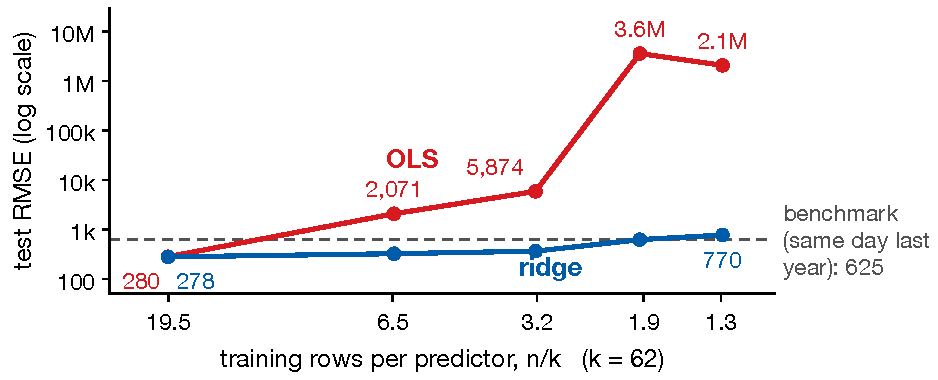
\includegraphics[height=4.4cm]{../Figures/Lecture06_Regularization/n_over_k.pdf}
  \end{center}
  \vspace{-0.3cm}
  {\small Same features, same test year. OLS goes from 280 to 3.6 million. Ridge, one line
  changed, ends at 770, a little worse than the benchmark.}
\end{frame}

% --- Slide: the fix ------------------------------------------------------------
\begin{frame}{Regularization: Fit Plus a Penalty}
  Three things go wrong as $k$ approaches $n$. The variance of $\hat{\boldsymbol{\beta}}$ grows
  with $k$. Correlated predictors get huge coefficients of opposite sign. Past $k > n$ there is no
  unique solution.

  \vspace{0.15cm}
  \textbf{Regularization} adds a penalty on coefficient size:
  \[
    \underbrace{\textstyle\sum_i (y_i - \hat{y}_i)^2}_{\text{fit}}
    + \underbrace{\lambda \cdot \text{Penalty}(\boldsymbol{\beta})}_{\text{complexity}}
  \]
  You accept a little bias for a large cut in variance. For a forecast, that trade is almost
  always worth making.
\end{frame}

% --- Slide: Subset selection -------------------------------------------------
\begin{frame}{Subset Selection: The Classical Answer}
  The classical approach \emph{counts} predictors rather than shrinking them
  \parencite{Guyon2003}.

  \vspace{0.15cm}
  \textbf{Best subset} fits all $2^k$ models: exact, and hopeless past $k \approx 30$.
  \textbf{Stepwise} adds or drops one predictor at a time: greedy, so it can miss the best
  combination. AIC, BIC or CV picks the winner \parencite[\S7.5]{Hyndman2021}.
  \begin{warningbox}
    Subset selection is \textbf{discrete}: a predictor is in or out, and small changes in the
    data flip it. The \emph{selected model} is itself high-variance --- the instability has
    moved somewhere harder to see.
  \end{warningbox}

  \vspace{0.1cm}
  \muted{\footnotesize Shrinkage replaces in-or-out with a continuous dial.}
\end{frame}

% =============================================================================
\section{Shrinkage Methods}
% =============================================================================

\sectionslide{Shrinkage Methods}{%
  Keep every predictor, but pull its coefficient toward zero.}

% --- Slide: Ridge ------------------------------------------------------------
\begin{frame}{Ridge Regression ($\ell_2$)}
  \begin{definitionbox}{Ridge \parencite{HoerlKennard1970}}
    \[
      \hat{\boldsymbol{\beta}}^{\text{ridge}}
      = \arg\min_{\boldsymbol{\beta}} \;
        \sum_{i=1}^{n}(y_i - \mathbf{x}_i'\boldsymbol{\beta})^2
        \; + \; \lambda \sum_{j=1}^{k} \beta_j^2
    \]
  \end{definitionbox}
  Ridge shrinks every coefficient toward zero and sets none exactly to zero: $\lambda = 0$ is
  OLS, and $\lambda \to \infty$ sends every $\beta_j \to 0$. Two correlated predictors split the
  effect between them instead of fighting over it.

  \vspace{0.15cm}
  \textbf{Use it when} most predictors carry a little signal and you want to keep them all.

  \vspace{0.15cm}
  \textbf{Standardize first.} The penalty is not scale-invariant: the same predictor in dollars
  and in thousands of dollars is penalized differently, and the units decide what survives.
\end{frame}

% --- Slide: LASSO ------------------------------------------------------------
\begin{frame}{LASSO ($\ell_1$)}
  \begin{definitionbox}{LASSO \parencite{Tibshirani1996}}
    \[
      \hat{\boldsymbol{\beta}}^{\text{lasso}}
      = \arg\min_{\boldsymbol{\beta}} \;
        \sum_{i=1}^{n}(y_i - \mathbf{x}_i'\boldsymbol{\beta})^2
        \; + \; \lambda \sum_{j=1}^{k} |\beta_j|
    \]
  \end{definitionbox}
  Swap the square for an absolute value and LASSO sets some coefficients \textbf{exactly} to
  zero: selection and estimation in one step, and a sparse model you can read aloud to a
  stakeholder.

  \vspace{0.15cm}
  \textbf{Use it when} only a handful of predictors genuinely matter and you want the model to
  say which.

  \vspace{0.15cm}
  \textbf{But be careful what you conclude.} Among highly correlated predictors LASSO keeps
  \emph{one}, more or less arbitrarily. The survivor is not ``the important one''; it won a coin
  toss between near-identical variables.
\end{frame}

% --- Slide: Why LASSO zeros out ----------------------------------------------
\begin{frame}{Why LASSO Zeros Out and Ridge Does Not}
  Both minimize squared error subject to a budget $t$: $\sum_j \beta_j^2 \le t$ or
  $\sum_j |\beta_j| \le t$. Ellipses of equal error grow from OLS until they touch the budget.
  Lab 6's lag7 and lag14, standardized:
  \begin{center}
    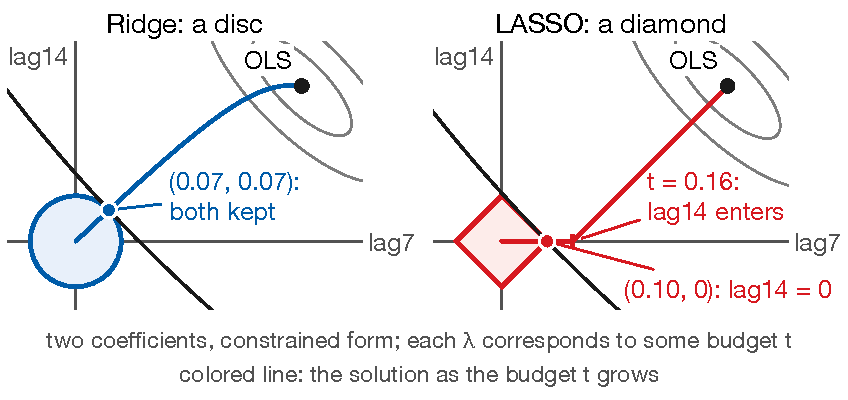
\includegraphics[height=4.3cm]{../Figures/Lecture06_Regularization/diamond_and_disc.pdf}
  \end{center}
  \vspace{-0.35cm}
  {\small The disc has no corners, so Ridge keeps both. The diamond's corner zeros lag14, but only
  while $t < 0.16$, a fifth of OLS's $\sum_j |\hat{\beta}_j| = 0.84$: these lags are nearly
  interchangeable, so the ellipses run almost along its face. A zero means ``not worth its budget
  here,'' not ``proven irrelevant'' \parencite[\S6.2]{James2021}.}
\end{frame}

% --- Slide: Elastic Net ------------------------------------------------------
\begin{frame}{Elastic Net: Both Penalties at Once}
  \begin{definitionbox}{Elastic Net \parencite{ZouHastie2005}}
    \[
      \sum_{i=1}^{n}(y_i - \mathbf{x}_i'\boldsymbol{\beta})^2
      \; + \; \lambda \left[ \alpha \sum_j |\beta_j|
      + (1-\alpha) \sum_j \beta_j^2 \right]
    \]
    $\lambda$ sets the total penalty; $\alpha \in [0,1]$ sets the mix ($\alpha=1$ is LASSO,
    $\alpha=0$ is Ridge).
  \end{definitionbox}
  The mix keeps LASSO's ability to zero out predictors while adding Ridge's \textbf{grouping
  effect}: correlated predictors now enter or leave together instead of one surviving
  arbitrarily.

  \vspace{0.15cm}
  \textbf{This is usually the right default for forecasting.} Lagged predictors are correlated
  almost by construction --- $y_{t-1}$ and $y_{t-2}$ move together --- which is precisely the
  situation where pure LASSO picks a winner at random and pure Ridge refuses to simplify.
\end{frame}

% --- Slide: the elastic-net ball ----------------------------------------------
% Figure: scripts/figures/lecture06_figures.py elastic_net (numbers in measured.json, "elastic_net").
\begin{frame}{The Grouping Effect, Drawn}
  The diamond again, beside the elastic-net ball at $\alpha = 0.5$, on the same ellipses and
  with the same reach along the axes:
  \begin{center}
    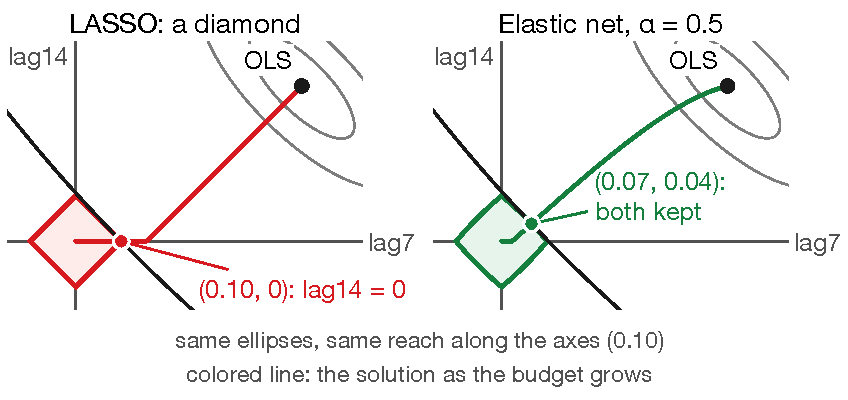
\includegraphics[height=4.3cm]{../Figures/Lecture06_Regularization/elastic_net.pdf}
  \end{center}
  \vspace{-0.35cm}
  {\small The ball is pointed only on the axes and curved everywhere else. At this budget the
  bend is slight, yet it moves the touch point off the corner. Its corner still zeros lag14, but
  only while the reach is below 0.02, against LASSO's 0.16.}
\end{frame}

% =============================================================================
\section{Choosing the Penalty}
% =============================================================================

\sectionslide{Choosing the Penalty}{%
  $\lambda$ is not estimated from the model. It is tuned --- and how you
  tune it decides whether the model generalizes.}

% --- Slide: Regularization path ----------------------------------------------
% Figure: scripts/figures/lecture06_figures.py lasso_path (Lab 6, Step 3; numbers in measured.json).
\begin{frame}{The Regularization Path}
  Fit across a grid of $\lambda$ and trace each coefficient: Lab 6's LASSO, all 62 features.
  They shrink, then drop to zero one at a time, until only the mean forecast is left.
  \begin{center}
    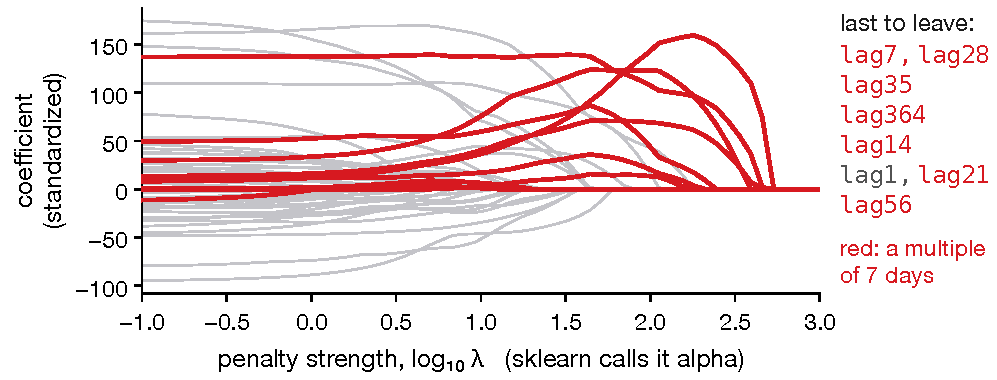
\includegraphics[height=4.2cm]{../Figures/Lecture06_Regularization/lasso_path.pdf}
  \end{center}
  \vspace{-0.35cm}
  {\small \textbf{The order in which predictors leave is the useful output.} Seven of the last
  eight are multiples of 7: the model also had day-of-week dummies, yet under heavy penalty it
  kept the weekly lags and dropped the dummies. Report that ordering, not one model's coefficient
  table.}
\end{frame}

% --- Slide: Choosing lambda --------------------------------------------------
\begin{frame}{Choosing $\lambda$ by Cross-Validation}
  \begin{enumerate}\small\itemsep0pt
    \item Define a grid of $\lambda$, usually log-spaced
    \item For each $\lambda$, run walk-forward CV, recording the mean validation RMSE
    \item Pick the $\lambda$ minimizing CV error, then refit on all training data
  \end{enumerate}

  \vspace{0.1cm}
  \textbf{The one-standard-error rule:} take the \emph{largest} $\lambda$ whose CV error is within
  one standard error of the minimum. You give up almost no accuracy for a simpler model.
  \begin{warningbox}
    \textbf{Default to \texttt{TimeSeriesSplit}}, as in Lecture 1. Random \texttt{KFold} trains
    on the future to validate the past: valid for a pure autoregression with uncorrelated errors
    \parencite{Bergmeir2018}, not under trend or serial correlation.
  \end{warningbox}
\end{frame}

% =============================================================================
\section{In Practice}
% =============================================================================

\sectionslide{In Practice}{%
  Standardize, tune on a time-aware split, and read the path.}

% --- Slide: Python -----------------------------------------------------------
\begin{frame}{Regularization in Python}
  \begin{examplebox}{Code Template}
    {\scriptsize
    \texttt{from sklearn.linear\_model import ElasticNetCV}\\
    \texttt{from sklearn.pipeline import make\_pipeline}\\
    \texttt{from sklearn.preprocessing import StandardScaler}\\
    \texttt{from sklearn.model\_selection import TimeSeriesSplit}\\[2pt]
    \texttt{model = make\_pipeline(StandardScaler(),}\\
    \texttt{\mbox{}\ \ ElasticNetCV(l1\_ratio=[.1,.5,.7,.9,.95,1],}\\
    \texttt{\mbox{}\ \ \ cv=TimeSeriesSplit(5), random\_state=42)).fit(X\_tr, y\_tr)}
    }
  \end{examplebox}
  \texttt{make\_pipeline} is the part that matters: it keeps standardization \emph{inside}
  each CV fold. Scale on the full sample and you have leaked the validation set into
  training, and your CV error is optimistic.

  \texttt{l1\_ratio} is the Ridge/LASSO mix; it equals $\alpha$ only at 0 and 1, since \texttt{sklearn}
  halves the $\ell_2$ term. \texttt{...CV} tunes $\lambda$, which \texttt{sklearn} calls \texttt{alpha}.
\end{frame}

% =============================================================================
\section{Key Takeaways and Roadmap}
% =============================================================================

\sectionslide{Key Takeaways and Roadmap}{%
  Shrinkage is the linear-model counterpart to what trees do by pruning.}

% --- Slide: Which method when -------------------------------------------------
\begin{frame}{Linear Methods: Which One When}
  \begin{center}
    {\small
    \begin{tabular}{llll}
      \toprule
      \textbf{Method} & \textbf{Penalty} & \textbf{Zeros out?} & \textbf{Best when} \\
      \midrule
      OLS & none & no & $k \ll n$, predictors uncorrelated \\
      Stepwise & discrete & yes & Few candidate predictors, need a story \\
      Ridge & $\ell_2$ & no & Many predictors, all mildly useful \\
      LASSO & $\ell_1$ & yes & Few predictors truly matter \\
      Elastic Net & both & yes & Many \emph{correlated} predictors \\
      \bottomrule
    \end{tabular}
    }
  \end{center}
  \vspace{0.15cm}
  \textbf{Connection to Lecture 5.} Trees and shrinkage solve the same problem in different
  geometries. XGBoost's \texttt{reg\_lambda} is literally a Ridge penalty on leaf weights
  (\texttt{reg\_alpha} is the LASSO one), and \texttt{gamma} charges a fixed price per leaf, like
  pruning's $\alpha$ in Lecture 4. Regularization is how every flexible model is kept honest.
\end{frame}

% --- Slide: Key takeaways ---------------------------------------------------
\begin{frame}{Lecture 6: Key Takeaways}
  \begin{keybox}
    {\footnotesize
    \begin{enumerate}\itemsep1pt
      \item With many predictors OLS overfits; past $k > n$ it has no unique solution.

      \item \textbf{Subset selection} is discrete, greedy and unstable.

      \item \textbf{Shrinkage} is a dial. Ridge shrinks all; LASSO's corners zero some, at
            small enough budgets; Elastic Net keeps correlated predictors together.

      \item \textbf{Standardize} inside each CV fold, and \textbf{tune $\lambda$} with
            \texttt{TimeSeriesSplit}, never random $K$-fold.

      \item The \textbf{regularization path}, the order predictors drop out, is more stable
            than any one coefficient table.
    \end{enumerate}
    }
  \end{keybox}
  \muted{\itshape Next: neural networks, where the fit-plus-penalty skeleton of Lectures 3--6
  returns as weight decay.}
\end{frame}

% --- References ---------------------------------------------------------------
\begin{frame}[allowframebreaks]{References}
  \renewcommand*{\bibfont}{\small}
  \printbibliography[heading=none]
\end{frame}

% =============================================================================
\end{document}
% =============================================================================
